\documentclass[11pt]{article}
\usepackage{lindrew}
\usepackage{amsfonts}
\usepackage{tikz}
\usetikzlibrary{automata, positioning, arrows}
\tikzset{
  ->,
  >=stealth,
  node distance=3cm,
  every state/.style={thick, fill=gray!10},
  initial text=$ $,
}
\usepackage{ulem}

\title{ECS 120: Theory of Computation}
\author{CptBreeza}

\begin{document}

\maketitle

\section{Alphabet, String and Language}

\subsection{Why}

In this course, we model an abstract computing machine with a function
$M : I \mapsto S$, where $I$ stands for \emph{inputs} and $S$ stands for
\emph{solutions}.

It is convenient to \emph{encode} both inputs and solutions as \emph{strings} over
a specific \emph{alphabet}. Consider problems called \emph{decision problems},
where there are only two elements in the solution set: \emph{true} or
\emph{false}, \emph{yes} or \emph{no}, $0$ or $1$. Thus, the inputs are
partitioned by the machine into two classes: those the machine gives a positive answer and those the machine gives a negative answer. We can collect all the
inputs which the machine gives positive answers into a set and we call this set a
language. And we begin our study of the theory of computation with the
definitions of \emph{alphabets}, \emph{strings} and \emph{languages}.

\subsection{Basic Concepts}

First, we define a \emph{language}:

\begin{definition}
A \emph{language} is a set of strings.
\end{definition}

That is pretty straightforward. A language can consist of no strings. A language can consist of an infinite number of strings. There's no requirements.

Next, we define a \emph{string}:
\begin{definition}
A \emph{string} is a finite sequence of characters.
\end{definition}

According to this definition, a string cannot be of infinite length. However, it can be empty. An empty string is typically denoted by $\epsilon$. The characters that make up a string are said to be drawn from an \emph{alphabet}:

\begin{definition}
An \emph{alphabet} is a finite nonempty set.
\end{definition}

We call an element of an alphabet a \emph{symbol}. We do not always specify the underlying alphabet.

\subsection{A Closer Look at Strings} \label{subsec:1.3}

A string has a nonnegative \emph{length}, which is defined as follows:
\begin{definition}
The \emph{length} of a string $A$ is:
\begin{enumerate}
\item $0$, if $A$ is an empty string.
\item $1 + n$, if $A$ is $c \cdot B$ and the length of $B$ is $n$.
\end{enumerate}
\end{definition}

In the definition above, we use capital letters for strings and lowercase letters for symbols.

This definition is an \emph{inductive definition}. After all, a string is nothing but a sequence of symbols (characters). We can always build a new string from an existing one by repeatedly attaching symbols to its head. To build new strings, there is always a starting string available even if we do not have any other string yet - the empty string $\epsilon$.

By thinking of strings as built from other strings, and considering that there is always a starting string $\epsilon$, we can classify strings into two types:
\begin{enumerate}
\item The empty string.
\item Strings that are built from other strings.
\end{enumerate}

Thus, we can simplify the definitions of functions over strings by exploiting this classification, as we did above in the definition of \emph{length}.

Of course, we can build new strings by concatenating existing strings:
\begin{definition}
The concatenation of two strings $A$ and $B$, $A \cdot B$, is:
\begin{enumerate}
\item $B$, if $A$ is $\epsilon$.
\item $a \cdot (A' \cdot B)$, if $A$ is $a \cdot A'$.
\end{enumerate}
\end{definition}

The dot notation $A \cdot B$ for concatenation is not chosen arbitrarily. It is similar to multiplication. It is \emph{associative}, so we can write $A \cdot B \cdot C$ without parentheses. The empty string $\epsilon$ acts like the number 1 in multiplication because, for any string $A$, both $A \cdot \epsilon$ and $\epsilon \cdot A$ are equal to $A$. It is easy to prove that $length(A \cdot B) = length(A) + length(B)$ for any strings $A$ and $B$.

We can also build a new string by reversing an existing one:
\begin{definition}
The reverse of a string $A$, $rev(A)$, is:
\begin{enumerate}
\item $\epsilon$, if $A$ is $\epsilon$.
\item $rev(A') \cdot a$, if $A$ is $a \cdot A'$.
\end{enumerate}
\end{definition}

It is true that for any strings $A$ and $B$, $rev(A \cdot B) = rev(B) \cdot rev(A)$.

\section{Languages, Deterministic Finite Automata}

\subsection{More on Languages}

To work with languages, we introduce an operation called \emph{Kleene star}:
\begin{definition}
The \emph{Kleene star} of a language $L$, denoted by $L^\ast$, is $\{x_1x_2x_3 \dots x_n | x_i \in L\}$.
\end{definition}

This definition is a little bit ambiguous. The ambiguity lies in the suspicious $\dots$. What if, say, $n$
is $0$?

To give a more rigorous definition, first we extend the concatenation operation of strings to languages:
\begin{definition}
The \emph{concatenation} of two languages $L_1$ and $L_2$, $L_1 \cdots L_2$, is $\{x \cdot y | x \in L_1 and y \in L_2\}$.
\end{definition}

And we define the \emph{power} of concatenation of languages:
\begin{definition}
For any nonnegative integer $n$ and any language $L$, $L^n$ is
\begin{enumerate}
\item $\{\epsilon\}$, if $n$ is $0$.
\item $L \cdot L^{n-1}$, if $n$ is greater than $0$.
\end{enumerate}
\end{definition}

We can define the \emph{Kleene star} of a language $L$ by powers of $L$:
\begin{definition}
$L^\ast = \bigcup_{n \in \mathbb{N}}L^n$.
\end{definition}

Now the ambiguity is resolved. According to the definition, it is clear that the empty string $\epsilon$ is
always in $L^\ast$ as a result of the case where $n$ is $0$.

By observing the preceding discussion, we find yet another way to define the \emph{Kleene star}:
\begin{definition}
$L^\ast$ is a set which
\begin{enumerate}
\item has $L$ as its subset.
\item is \emph{closed} under concatenation.
\end{enumerate}
\end{definition}

\subsection{Deterministic Finite Automata}

We might have seen a (finite) state machine before. A \emph{finite state machine (FSM)}, which we call
\emph{Deterministic Finite Automaton (DFA)} in this course, is a facility which
\begin{enumerate}
\item stores a state.
\item accepts inputs.
\item may move (transition) to another state under certain inputs.
\end{enumerate}

It can be used to test if a string has certain \emph{pattern}. For example, consider the DFA shown below:
\begin{figure}[ht]
    \centering
    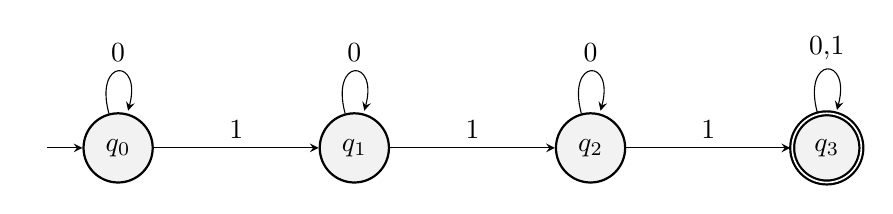
\begin{tikzpicture}
      \node[state,initial] (q0) {$q_0$};
      \node[state,right of=q0] (q1) {$q_1$};
      \node[state,right of=q1] (q2) {$q_2$};
      \node[state,accepting,right of=q2] (q3) {$q_3$};

      \draw (q0) edge[loop above] node{0}   (q0)
            (q0) edge[above]      node{1}   (q1)
            (q1) edge[loop above] node{0}   (q1)
            (q1) edge[above]      node{1}   (q2)
            (q2) edge[loop above] node{0}   (q2)
            (q2) edge[above]      node{1}   (q3)
            (q3) edge[loop above] node{0,1} (q3);
    \end{tikzpicture}
    \caption{a simple DFA}
    \label{fig:fig1}
\end{figure}

From the diagram, we can infer that the underlying alphabet is $\{0, 1\}$ and this DFA \emph{accepts} strings
that consist of at least three $1$s.

We define a DFA formally as follows:
\begin{definition}
A \emph{Finite Deterministic Automaton}, $M$, is a tuple $\{Q, \Sigma, \delta, q_0, F\}$ where:
\begin{itemize}
\item $Q$ is a finite nonempty set of \emph{states}.
\item $\Sigma$ is the alphabet of the inputs.
\item $\delta: Q \times \Sigma \mapsto Q$ is a transition function which specifies how states are changed over
inputs.
\item $q_0 \in Q$ is the initial state.
\item $F \subseteq Q$ is the set of accept states.
\end{itemize}
\end{definition}

As a DFA \emph{accepts} some strings but reject others, we can partition a language with it. Furthermore,
strings which a DFA $M$ accepts form a language $L$:
\begin{definition}
The set of all strings that a DFA $M$ accepts, $M$, is a language. We denote it by $L(M)$.
\end{definition}

What does it mean for a DFA to \emph{accept} a string? First, we define an auxiliary function $\delta ^ \ast$ - an
extension of the function $\delta$ shown above:
\begin{definition}
The function $\delta ^ \ast : Q \times \Sigma ^ \ast \mapsto Q$ maps a state and a string to another state.

For any state $q$ and string $s$, $\delta ^ \ast (q, s)$ is:
\begin{enumerate}
\item $q$, if $s$ is the empty string $\epsilon$.
\item $\delta ^ \ast( \delta(q, a), s' )$, if $s$ is $a \cdot s'$.
\end{enumerate}
\end{definition}

Then, with this definition, we say that a DFA $M$ accepts a string $s$ iff $\delta ^ \ast(q_0, s) \in F$.

\section{Building DFAs} \label{sec:3}

\subsection{Example 1: Can We Build a Smaller DFA?} \label{subsec:3.1}

What we want: build a DFA accept the language $\{s \in \{a,b\} ^\ast \mid \text{s
does not end with "bbb"} \}$.

How can we build it: instead of thinking about "not end with", first we build a DFA which accepts strings that end with "bbb". And then we "negate" it by turning the
accept states into non-accept states and non-accept states into accept states.
That is pretty straightforward. First, we build the DFA as shown in \ref{fig:fig2}.

\begin{figure}[ht]
    \centering
    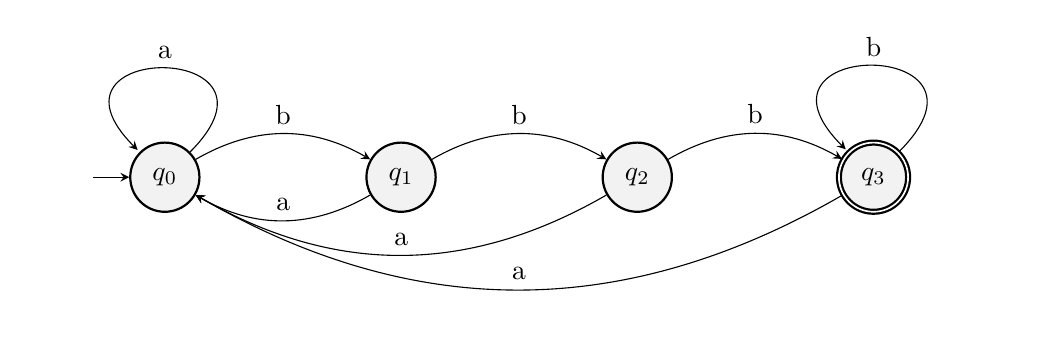
\begin{tikzpicture}
      \node[state,initial] (q0) {$q_0$};
      \node[state,right of=q0] (q1) {$q_1$};
      \node[state,right of=q1] (q2) {$q_2$};
      \node[state,accepting,right of=q2] (q3) {$q_3$};

      \draw (q0) edge[loop,above]           node{a}   (q0)
            (q0) edge[bend left,above]      node{b}   (q1)
            (q1) edge[bend left,above]      node{a}   (q0)
            (q1) edge[bend left,above]      node{b}   (q2)
            (q2) edge[bend left,above]      node{a}   (q0)
            (q2) edge[bend left,above]      node{b}   (q3)
            (q3) edge[bend left,above]      node{a}   (q0)
            (q3) edge[loop,above]           node{b}   (q3);
    \end{tikzpicture}
    \caption{a DFA which accepts all strings that end with "bbb"}
    \label{fig:fig2}
\end{figure}

Then, we negate the states to get the desired DFA:

\begin{figure}[ht]
    \centering
    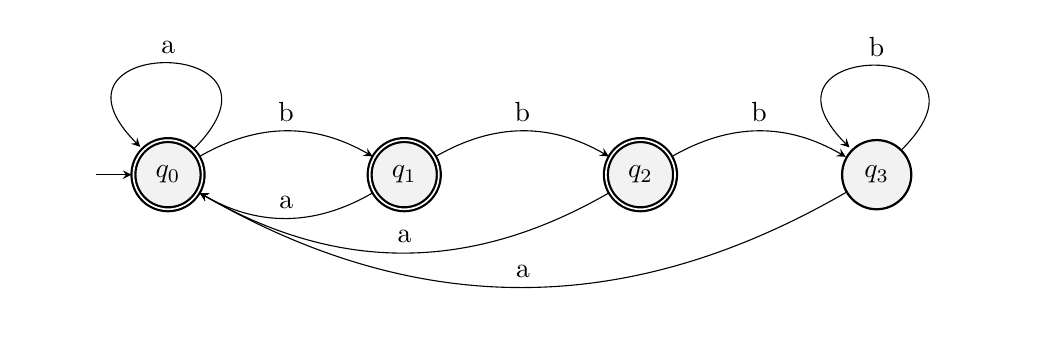
\begin{tikzpicture}
      \node[state,initial,accepting] (q0) {$q_0$};
      \node[state,accepting,right of=q0] (q1) {$q_1$};
      \node[state,accepting,right of=q1] (q2) {$q_2$};
      \node[state,right of=q2] (q3) {$q_3$};

      \draw (q0) edge[loop,above]           node{a}   (q0)
            (q0) edge[bend left,above]      node{b}   (q1)
            (q1) edge[bend left,above]      node{a}   (q0)
            (q1) edge[bend left,above]      node{b}   (q2)
            (q2) edge[bend left,above]      node{a}   (q0)
            (q2) edge[bend left,above]      node{b}   (q3)
            (q3) edge[bend left,above]      node{a}   (q0)
            (q3) edge[loop,above]           node{b}   (q3);
    \end{tikzpicture}
    \caption{a DFA which accepts all strings that do not end with "bbb"}
    \label{fig:fig3}
\end{figure}

Can we build a DFA accepting the same language but with fewer states? Or, if stated in another way, is this DFA a \emph{minimal} one? I don't think so. The intuition is
this: since we want to filter (or filter out) all strings that end with "bbb", we
need to count how many "b"s are there right before the inputs are exhausted. And for
DFAs, this count is remembered, or encoded, by states. We need four states to
represent possible counts that can distinguish different situations, where the
string is one "b" from being accepted, two "b"s from being accepted, three "b"s from
being accepted and is already acceptable.

Can we prove it? Surely we can. We prove it by the \emph{Pigeonhole Principle}.

\begin{proof}
We prove this by contradiction. Assume that we \emph{can} build such a DFA $M$
with three states. Now consider following strings:
\begin{align*}
&\epsilon \\
&b \\
&bb \\
&bbb
\end{align*}

Or more compactly, the strings $b^i$ where $0 \leq i \leq 3$. There are four of
them. We feed them into $M$ and we get four states $\delta ^ \ast(q_0, b^i)$.
Since $M$ has three states and there are four states produced, by the
Pigeonhole Principle, at least two of the produced states are the same one.

Let us check it. We pick two strings $b^i$ and $b^I$, where $0 \leq i < I
\leq 3$. We feed them into of $M$. The states produced after that are $\delta ^
\ast(q_0, b^i)$ and $\delta ^ \ast(q_0, b^I)$. But we do not stop here. We then feed
the string $b^{3-I}$. And that produces states $\delta ^ \ast(q_0, b^{i + 3 - I})$
and $\delta ^ \ast(q_0, b^3)$. Are they the same state? The state $\delta ^
\ast(q_0, b^3)$ is an accept state. Since $i < I$, $i + 3 - I$ is strictly less
than $3$. That implies that state $\delta ^ \ast(q_0, b^{i + 3 - I})$ is not an
accept state. These states are distinct.

We have now proved that for any two of the four strings listed above, the states
produced after feeding them into $M$ are distinct. That is to say that $M$ has
at least four distinct states. This contradicts our original hypothesis that
$M$ has three states. So we cannot build such a DFA with three states.
\end{proof}

\subsection{Example 2: Can We Build That DFA At All?}

What we want: build a DFA accepting the language $\{s \in \{a,b\}^\ast \mid a^nb^n
, n \in \mathbb{N}\}$.

How can we build it: I don't think we can build it. As we have seen in the example
in \ref{subsec:3.1}, states of DFAs can remember, or encode, certain information.
But as the name of DFA suggests, there is only a finite amount of information can
be stored by the finite states. To accept the language shown above, however, requires
the machine to remember an indefinite amount of information. That cannot be done
with a finite number of states.

Can we prove it? Surely we can. We prove it by the Pigeonhole Principle.

\begin{proof}
We prove this by contradiction. Assume that we \emph{can} build such a DFA $M$ with
$me$ states. Now consider following strings:
\begin{align*}
&\epsilon \\
&a^mb \\
&a^mb^2 \\
&\dots \\
&a^mb^m
\end{align*}
Or more compactly, the strings $a^mb^i$ where $0 \leq i \leq m$. There are $m + 1$ of
them. We feed them into $M$ and we get $m + 1$ states $\delta ^ \ast(q_0, a^mb^i)$.
Since $M$ has $m$ states and there are $m + 1$ states produced, by the Pigeonhole
Principle, at least two of the produced states are the same one.

Let us check it. We pick two strings $b^i$ and $b^I$, where $0 \leq i < I \leq m$. We
feed them into $M$. The states produced after that are $\delta ^ \ast(q_0, a^mb^i)$
and $\delta ^ \ast(q_0, a^mb^I)$. But we do not stop here. We then feed the string
$b^{m-I}$. And that produces states $\delta ^ \ast(q_0, b^{i + m - I}$ and
$\delta ^ \ast(q_0, b^m)$. Are they the same state? The state
$\delta ^ \ast(q_0, b^m)$ is an accept state. Since $i < I$, $i + m - I$ is
strictly less than $m$. That implies that the state
$\delta ^ \ast(q_0, b^{i + m - I}$ is not an accept state. These states are
distinct.

We have now proved that for any two of the four strings listed above, the states
produced after feeding them into $M$ are distinct. That is to say that $M$ has at
least $m + 1$ distinct states. This contradicts our original hypothesis that $M$ has
$m$ states. So we cannot build such a DFA.
\end{proof}

There are languages which cannot be accept by any DFA. And the reason of this is that
DFA is not powerful enough.

\subsection{Can We Build new DFAs Systematically From Exising Ones?} \label{subsec:3.3}

What we want: As discussed in \ref{subsec:1.3}, we can build new strings from
existing ones by concatenation and reversal. Similarly, we want some systematical
methods to build DFAs from existing ones.

How we can build it: It is not easy to compose DFAs. While we developed a connection
between languages and DFAs. Languages are sets. We instead consider following
questions:
Assume there are DFAs that can accept $L_1$ and $L_2$.
\begin{enumerate}
\item Is there a DFA that accept $\overline{L_1}$?
\item Is there a DFA that accept $L_1 \cup L_2$?
\item Is there a DFA that accept $L_1 \cap L_2$?
\end{enumerate}

\subsubsection{Complement}

As we see in the example in \ref{subsec:3.1}, where we build a DFA and then negate
it. It is obvious that we can always build a new DFA from an existing one by negating
all its states.

\subsubsection{Union} \label{subsubsec:3.3.2}

It is possible to build a DFA accepting $L_1 \cup L_2$.

Imagine that $L_1$ is at our left hand and $L_2$ is at our right hand. As the input
symbols are fed, we move hands following the transitions respectively in the two DFAs. After all inputs are fed, each of our hands would point to a state. If either
the final states pointed is an accept state, then we say that the new DFA accept
the input. And this DFA accepts $L_1 \cup L_2$.

Let us construct it formally.
\begin{definition}
Assume that there are two machines $M_1=\{Q_1,\Sigma,\delta_1,q_1,F_1\}$ and
$M_2 = \{Q_2, \Sigma,\delta_2,q_2,F_2\}$. They accepts $L_1$ and $L_2$ respectively.
The machine $M = \{Q,\Sigma,\delta,q_0,F\}$ accepting $L_1 \cup L_2$ can be
constructed as follows:
\begin{enumerate}
\item $Q = Q_1 \times Q_2$
\item $\Sigma$ = $\Sigma$
\item $\delta(q, s) = (\delta_1(q_1, s), \delta_2(q_2, s))$ where $q = (q_1, q_2)$
\item $q_0 = (q_1, q_2)$
\item $F = \{q \in Q \mid q_1 \in F_1 \vee q_2 \in F_2\}$
\end{enumerate}
\end{definition}

The construction defined above is often called a \emph{product machine}, since the
number of states of it is the product of the two building DFAs.

\subsubsection{Intersection}

It is possible to build a DFA accepting $L_1 \cap L_2$.

In fact, we can employ the same construction that we build in \ref{subsubsec:3.3.2}
- the product machine - to build this DFA. All is same but $F$. In this case, $F$
should be $\{q \in Q \mid q_1 \in F_1 \wedge q_2 \in F2\}$.

There is another way to build this DFA by exploiting the \emph{De Morgan's Law}.
That is $L_1 \cap L_2 = \overline{\overline{L_1} \cup \overline{L_2}}$.

\section{Nondeterministic Finite Automata} \label{sec:4}

As shown in \ref{subsec:3.3}, given $L_1 = L(M_1)$ and $L_2 = L(M_2)$, there exists
$M$ that accepts
\begin{enumerate}
\item $\overline{L_1}$
\item $L_1 \cup L_2$
\item $L_1 \cap L_2$
\end{enumerate}

We have discussed two operations $L_1 \cdot L_2$ and $L^\ast$ but they are not on
this list. Can we build a DFA that accepts $L_1 \cdot L_2$ or $L^\ast$?

\subsection{Can We Build new DFAs Systematically From Existing Ones? Cont.}

\subsubsection{Concatenation} \label{subsubsec:4.1.1}

For a machine to accept $L(M_1) \cdot L(M_2)$, we need to

\begin{enumerate}
\item wire up the accept states of $M_1$ to the initial state of $M_2$
\item turn the accept states of $M_1$ to nonaccept states
\end{enumerate}

Then, for any string to reach the accept states of the resultant machine, it must go
through first $M_1$ and then $M_2$. This is exactly what we want for a machine to
accept $L_1 \cdot L_2$.

Here is an example. $M_1$ accepts $L_1$, which is the language of all strings that start
with "bb":

\begin{figure}[ht]
    \centering
    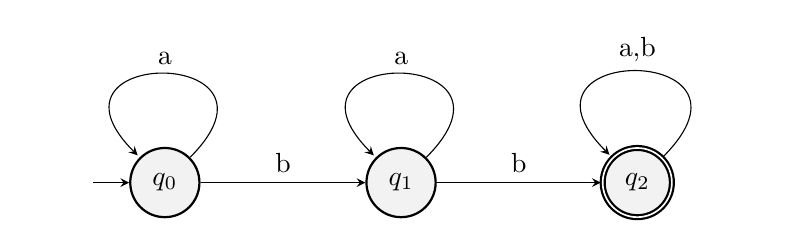
\begin{tikzpicture}
      \node[state,initial]               (q0) {$q_0$};
      \node[state,right of=q0]           (q1) {$q_1$};
      \node[state,accepting,right of=q1] (q2) {$q_2$};

      \draw (q0) edge[loop,above]           node{a}   (q0)
            (q0) edge[above]                node{b}   (q1)
            (q1) edge[loop,above]           node{a}   (q1)
            (q1) edge[above]                node{b}   (q2)
            (q2) edge[loop,above]           node{a,b} (q2);
    \end{tikzpicture}
    \caption{a DFA which accepts all strings that start with "bb"}
    \label{fig:fig4}
\end{figure}

$M_2$ accepts $L_2$, which is the language of all strings that end with "aa":

\begin{figure}[ht]
    \centering
    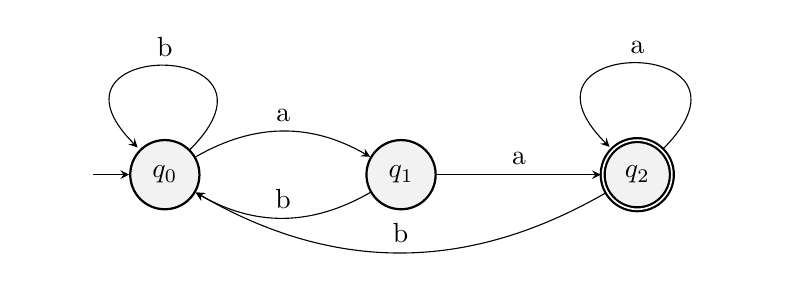
\begin{tikzpicture}
      \node[state,initial]               (q0) {$q_0$};
      \node[state,right of=q0]           (q1) {$q_1$};
      \node[state,accepting,right of=q1] (q2) {$q_2$};

      \draw (q0) edge[loop,above]           node{b} (q0)
            (q0) edge[bend left,above]      node{a} (q1)
            (q1) edge[bend left,above]      node{b} (q0)
            (q1) edge[above]                node{a} (q2)
            (q2) edge[loop,above]           node{a} (q2)
            (q2) edge[bend left,above]      node{b} (q0);
    \end{tikzpicture}
    \caption{a DFA which accepts all strings that end with "aa"}
    \label{fig:fig5}
\end{figure}

Below is a DFA which accepts $L_1 \cdot L_2$:

\begin{figure}[ht]
    \centering
    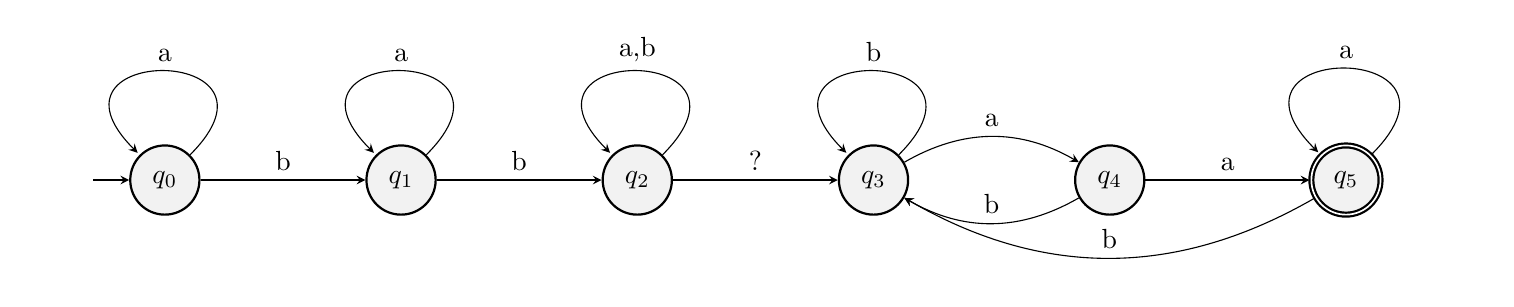
\begin{tikzpicture}
      \node[state,initial]               (q0) {$q_0$};
      \node[state,right of=q0]           (q1) {$q_1$};
      \node[state,right of=q1]           (q2) {$q_2$};
      \node[state,right of=q2]           (q3) {$q_3$};
      \node[state,right of=q3]           (q4) {$q_4$};
      \node[state,accepting,right of=q4] (q5) {$q_5$};

      \draw (q0) edge[loop,above]           node{a}   (q0)
            (q0) edge[above]                node{b}   (q1)
            (q1) edge[loop,above]           node{a}   (q1)
            (q1) edge[above]                node{b}   (q2)
            (q2) edge[above]                node{?}   (q3)
            (q2) edge[loop,above]           node{a,b} (q3)
            (q3) edge[loop,above]           node{b}   (q3)
            (q3) edge[bend left,above]      node{a}   (q4)
            (q4) edge[bend left,above]      node{b}   (q3)
            (q4) edge[above]                node{a}   (q5)
            (q5) edge[loop,above]           node{a}   (q5)
            (q5) edge[bend left,above]      node{b}   (q3);
    \end{tikzpicture}
    \caption{a \sout{DFA} which accepts all strings that start with "bb" and end with "aa"}
    \label{fig:fig6}
\end{figure}

It seems to be working fine, except the transition from $q_2$ to $q_3$.
As the question mark above the transition line in the diagram suggests,
there is no symbol from the alphabet (which is, inferred from context,
$\{a,b\}$) that could do the job.

So, why not introduce a special purpose symbol for convenience? To be
specific, we can introduce a symbol, $\epsilon$, to indicate that the
transition can be made with no input symbol at all. The notation is
not a coincidence. In previous discussion, we use $\epsilon$ to denote
the empty string. Here, $\epsilon$ means \emph{nothing},
\emph{empty symbol}.

Let us fix figure \ref{fig:fig6} by putting replacing the "?" with
$\epsilon$:

\begin{figure}[ht]
    \centering
    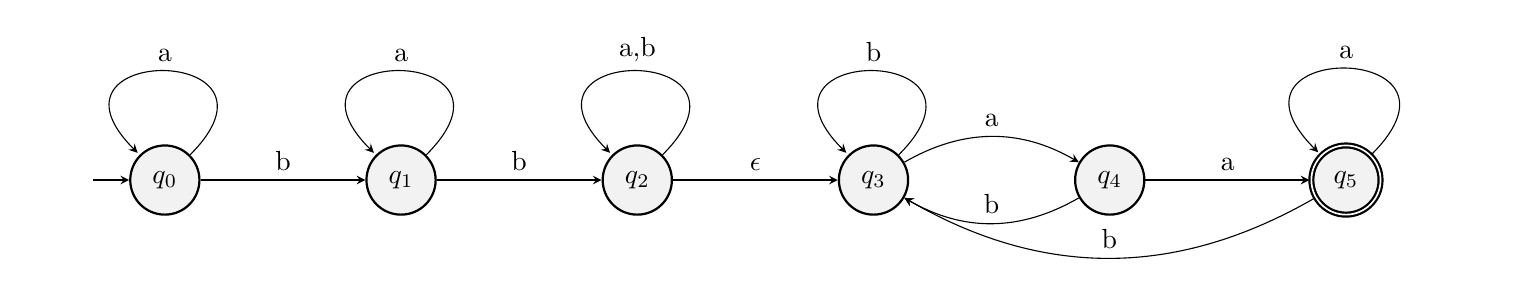
\begin{tikzpicture}
      \node[state,initial]               (q0) {$q_0$};
      \node[state,right of=q0]           (q1) {$q_1$};
      \node[state,right of=q1]           (q2) {$q_2$};
      \node[state,right of=q2]           (q3) {$q_3$};
      \node[state,right of=q3]           (q4) {$q_4$};
      \node[state,accepting,right of=q4] (q5) {$q_5$};

      \draw (q0) edge[loop,above]           node{a}   (q0)
            (q0) edge[above]                node{b}   (q1)
            (q1) edge[loop,above]           node{a}   (q1)
            (q1) edge[above]                node{b}   (q2)
            (q2) edge[above]                node{$\epsilon$}   (q3)
            (q2) edge[loop,above]           node{a,b} (q3)
            (q3) edge[loop,above]           node{b}   (q3)
            (q3) edge[bend left,above]      node{a}   (q4)
            (q4) edge[bend left,above]      node{b}   (q3)
            (q4) edge[above]                node{a}   (q5)
            (q5) edge[loop,above]           node{a}   (q5)
            (q5) edge[bend left,above]      node{b}   (q3);
    \end{tikzpicture}
    \caption{an NFA which accepts all strings that start with "bb" and end with "aa" fixed}
    \label{fig:fig7}
\end{figure}

This machine, with a transition labeled by $\epsilon$, is no longer
a DFA. If the machine is at state $q_2$, and we feed an $a$ into it,
it can stay at $q_2$ or transition to $q_4$. Why $q_4$? The machine
is not \emph{stable}, or not deterministic, at $q_2$ in the presence
of the $\epsilon$ transition, in the sense that it is actually at
both $q_2$ and $q_3$. If it is at $q_2$, it would transition to
$q_2$. If it is at $q_3$, it would transition to $q_4$.

The key difference between this machine and a DFA is that with an
input there is only one path possible in a DFA, but many paths in
this machine. By this feature, we call this machine a
\emph{nondeterministic finite automaton (NFA)}.

What is for an NFA to accept a string? For a DFA, it accepts a string
as long as \emph{the} path leads to an accept state. For a NFA, since
there are many paths possible, it accepts a string as long as there is
\emph{a} path that leads to an accept state.

Now, We have shown that with the introduction of the $\epsilon$
transition, we can build an NFA $M$ out of DFAs $M_1$ and $M_2$
that accepts $L = L_1 \cdot L_2$. This is not what we are asking
for. We are asking for a DFA but instead got an NFA. In latter
discussions, we will show that we can build a DFA that accepts
exactly the same language out of an NFA. And that is to say
that we can build a DFA that accepts $L_1 \cdot L_2$.

\subsubsection{Kleene Star}

To build a DFA or an NFA that accepts $L^\ast$, we employ a strategy
similar to the one we used in section \ref{subsubsec:4.1.1}. That is,
for $L^\ast$, we

\begin{enumerate}
\item wire up the accept states of $M$ to its own initial state
\item turn the initial state to an accept state
\end{enumerate}

Here is an example. $L$ is the language of all strings that start with "bb".
$L^\ast$ contains all strings that start with "bb" and the empty string $\epsilon$.
Following the instruction above, we can bulid an NFA for $L^\ast$. The diagram
of $M$ is shown in figure \ref{fig:fig8}.

\begin{figure}[ht]
    \centering
    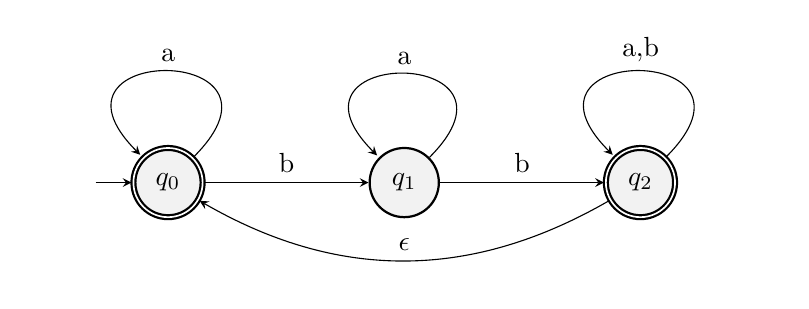
\begin{tikzpicture}
      \node[state,initial,accepting]     (q0) {$q_0$};
      \node[state,right of=q0]           (q1) {$q_1$};
      \node[state,accepting,right of=q1] (q2) {$q_2$};

      \draw (q0) edge[loop,above]           node{a}   (q0)
            (q0) edge[above]                node{b}   (q1)
            (q1) edge[loop,above]           node{a}   (q1)
            (q1) edge[above]                node{b}   (q2)
            (q2) edge[loop,above]           node{a,b} (q2)
            (q2) edge[bend left,above]           node{$\epsilon$} (q0);
    \end{tikzpicture}
    \caption{an NFA that is supposed to accept $L^\ast$ where $L$ is the language
    of all strings that start with "bb"}
    \label{fig:fig8}
\end{figure}

It almost works, except that it is problematic to turn the initial state to an
accept state. Consider the example of $M$ , shown in figure \ref{fig:fig9},
that accepts $L^\ast$ where $L$ is the language of all strings that end with
"aa". If we turn $q_0$ to an accept state, a string like "baab" would be
accepted by $M$. This is certainly not what we want.

\begin{figure}[ht]
    \centering
    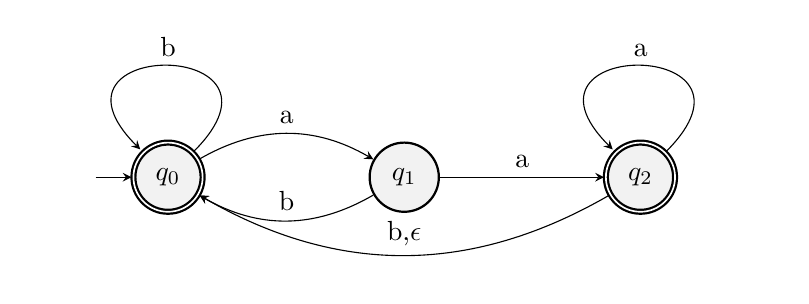
\begin{tikzpicture}
      \node[state,initial,accepting]     (q0) {$q_0$};
      \node[state,right of=q0]           (q1) {$q_1$};
      \node[state,accepting,right of=q1] (q2) {$q_2$};

      \draw (q0) edge[loop,above]           node{b} (q0)
            (q0) edge[bend left,above]      node{a} (q1)
            (q1) edge[bend left,above]      node{b} (q0)
            (q1) edge[above]                node{a} (q2)
            (q2) edge[loop,above]           node{a} (q2)
            (q2) edge[bend left,above]      node{b,$\epsilon$} (q0);
    \end{tikzpicture}
    \caption{an NFA that is supposed to accept $L^\ast$ where $L$ is the language
    of all strings that end with "aa"}
    \label{fig:fig9}
\end{figure}

To fix things up, we need an extra state, which is to be the new initial state.
And the accept states should wire up to this extra state. To be specific, we
need to:
\begin{enumerate}
\item add a new state and make it the new initial state and an accept state
\item add a $\epsilon$ transition from the new initial state to the original
initial state
\item add $\epsilon$ transitions from accept states to the new initial state
\end{enumerate}

$M$ fixed is shown below in figure \ref{fig:fig10}.

\begin{figure}[ht]
    \centering
    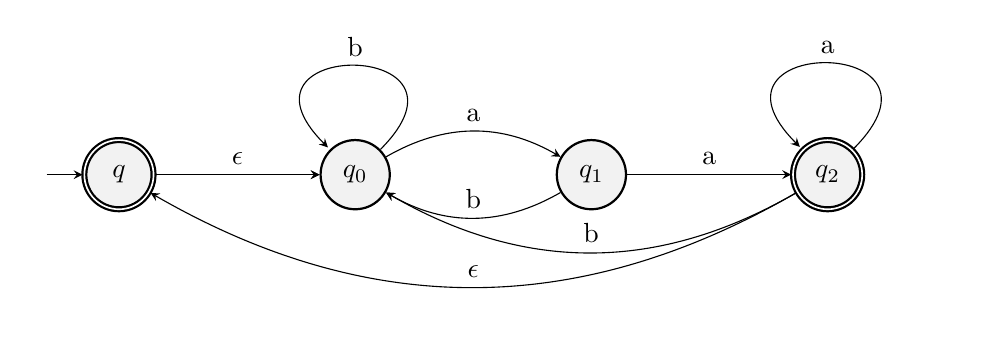
\begin{tikzpicture}
      \node[state,initial,accepting]     (q)  {$q$};
      \node[state,initial,right of=q]    (q0) {$q_0$};
      \node[state,right of=q0]           (q1) {$q_1$};
      \node[state,accepting,right of=q1] (q2) {$q_2$};

      \draw (q)  edge[above]                node{$\epsilon$} (q0)
            (q0) edge[loop,above]           node{b} (q0)
            (q0) edge[bend left,above]      node{a} (q1)
            (q1) edge[bend left,above]      node{b} (q0)
            (q1) edge[above]                node{a} (q2)
            (q2) edge[loop,above]           node{a} (q2)
            (q2) edge[bend left,above]      node{b} (q0)
            (q2) edge[bend left,above]      node{$\epsilon$} (q);
    \end{tikzpicture}
    \caption{an NFA that accepts $L^\ast$ where $L$ is the language of all
    strings that end with "aa"}
    \label{fig:fig10}
\end{figure}

Now, we have shown that we can build an NFA $M'$ that accepts $L^\ast$ out of
a DFA $M$. Again, this is not what we are asking for. We are asking for a DFA
but instead got an NFA.

\subsection{Defining Nondeterministic Finite Automata}

In fact, in addition to the $\epsilon$ transition, there are two more features
of NFA:
\begin{enumerate}
\item we do not have to exhaust all symbols of the alphabet for outgoing
transitions of a state
\item there can be more than one possible transitions from one state under an input
\end{enumerate}

These two features can be demonstrated in the following example:

\begin{figure}[ht]
    \centering
    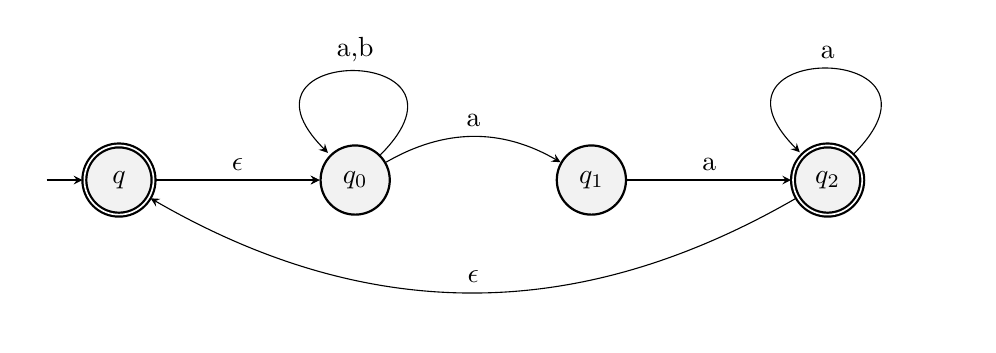
\begin{tikzpicture}
      \node[state,initial,accepting]     (q)  {$q$};
      \node[state,initial,right of=q]    (q0) {$q_0$};
      \node[state,right of=q0]           (q1) {$q_1$};
      \node[state,accepting,right of=q1] (q2) {$q_2$};

      \draw (q)  edge[above]                node{$\epsilon$} (q0)
            (q0) edge[loop,above]           node{a,b} (q0)
            (q0) edge[bend left,above]      node{a} (q1)
            (q1) edge[above]                node{a} (q2)
            (q2) edge[loop,above]           node{a} (q2)
            (q2) edge[bend left,above]      node{$\epsilon$} (q);
    \end{tikzpicture}
    \caption{an NFA that accepts $L^\ast$ where $L$ is the language of all
    strings that end with "aa"}
    \label{fig:fig11}
\end{figure}

As we can see, the alphabet in this example is $\{a,b\}$. There are no outgoing
transitions from $q_1$ labeled $b$. And from $q_0$, there are two outgoing
transitions labeled $a$, one to $q_0$ and another to $q_1$.

\subsubsection{NFA can be non-exhaustive}

If a symbol is fed, and there are no transitions outgoing labeled with it,
we might think that the machine transitions to a "dead" state. It is a trap
where there is no input can take the machine out of it. Below is an example
of figure \ref{fig:fig11} with an explicit "dead" state.

\begin{figure}[ht]
    \centering
    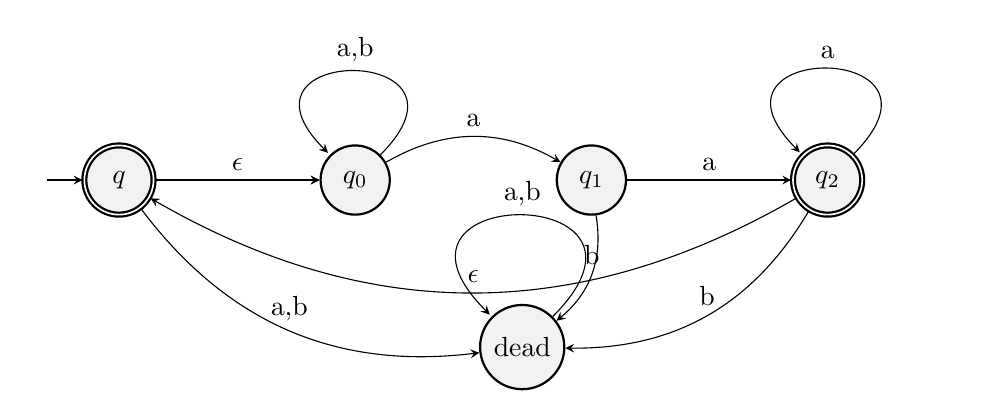
\begin{tikzpicture}
      \node[state,initial,accepting]     (q)  {$q$};
      \node[state,initial,right of=q]    (q0) {$q_0$};
      \node[state,right of=q0]           (q1) {$q_1$};
      \node[state,accepting,right of=q1] (q2) {$q_2$};
      \node[state,below right of=q0]     (dead) {dead};

      \draw (q)  edge[above]               node{$\epsilon$} (q0)
            (q0) edge[loop,above]          node{a,b} (q0)
            (q0) edge[bend left,above]     node{a} (q1)
            (q1) edge[above]               node{a} (q2)
            (q2) edge[loop,above]          node{a} (q2)
            (q2) edge[bend left,above]     node{$\epsilon$} (q)
            (q)  edge[bend right,above]    node{a,b} (dead)
            (q1) edge[bend left,above]     node{b} (dead)
            (q2) edge[bend left,above]     node{b} (dead)
            (dead) edge[loop,above]        node{a,b} (dead);
    \end{tikzpicture}
    \caption{an NFA with an explicit "dead" state}
    \label{fig:fig12}
\end{figure}

\subsubsection{NFA Transitions From One State to Several States}

With $\epsilon$ transitions and the ability to draw several outgoing
transitions from a state of a label, an NFA transitions from one state
to several states.

Here is an example. Let us find out all transitions in the example:

\begin{figure}[ht]
    \centering
    \begin{tikzpicture}
      \node[state,initial,right of=q]    (q0) {$q_0$};
      \node[state,right of=q0]           (q1) {$q_1$};
      \node[state,accepting,right of=q1] (q2) {$q_2$};

      \draw (q0) edge[loop,above]           node{a,b} (q0)
            (q0) edge[bend left,above]      node{a} (q1)
            (q1) edge[above]                node{a} (q2)
            (q1) edge[bend left,above]      node{a} (q0)
            (q2) edge[loop,above]           node{a} (q2);
    \end{tikzpicture}
    \caption{}
    \label{fig:fig13}
\end{figure}

\begin{align*}
&\delta(q_0, a) = \{q_0,q_1\} \\
&\delta(q_0, b) = \{q_0\} \\
&\delta(q_1, a) = \{q_0,q_2\} \\
&\delta(q_1, b) = \emptyset \\
&\delta(q_2, a) = \{q_1\} \\
&\delta(q_2, b) = \emptyset
\end{align*}

\subsubsection{Formal Definition}

After examining the behaviours, we can finally formally define a NFA:
\begin{definition}
A \emph{Nondeterministic Finite Automaton}, $M$, is a tuple $\{Q,\Sigma,\delta,q_0,F\}$ where:
\begin{itemize}
\item $Q$ is a finite nonempty set of states
\item $\Sigma$ is the alphabet of the inputs
\item $\delta : Q \times (\Sigma \cup \{\epsilon\}) \mapsto \mathcal{P}(Q)$
\item $q_0 \in Q$ is the initial state
\item $F \subseteq Q$ is the set of accept states
\end{itemize}
\end{definition}

And what does it mean for an NFA to accept a string:
\begin{definition}
An NFA $M = \{Q,\Sigma,\delta,q_0,F\}$ accepts a string $s$ \\
if there exists
$a_1,a_2,\dots,a_n \in (\Sigma \cup \{\epsilon\})$ and
$q_q,q_2,\dots,q_n \in Q$ where \\
$s = a_1 a_2 \dots a_n$ and \\
$q_i = \delta(q_{i-1},a_i)$ for all $1 \leq i \leq n$ and \\
$q_n \in F$.
\end{definition}

\section{DFA/NFA equivalence, Regular Language and Regular Expression}

\subsection{Build a DFA out of an NFA by Grouping States} \label{subsec:5.1}

Now it is time to show that every NFA can be turned into a DFA. Let us do this by first
show an example. Consider an NFA $M$ as shown below:

\begin{figure}[ht]
    \centering
    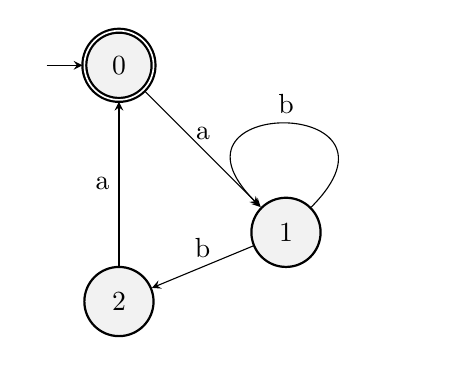
\begin{tikzpicture}
      \node[state,initial,accepting]  (q0) {0};
      \node[state,below right of=q0]  (q1) {1};
      \node[state,below of=q0]        (q2) {2};

      \draw (q0) edge[above]      node{a} (q1)
            (q1) edge[loop,above] node{b} (q1)
            (q1) edge[above]      node{b} (q2)
            (q2) edge[left]       node{a} (q0);
    \end{tikzpicture}
    \caption{}
    \label{fig:fig14}
\end{figure}

We will draw a table of all transitions of $M$. But this time we do it in a slightly
different way. First, instead of $0$, we use $\{0\}$ as the initial state. Then, we
figure out which set of states it transitions to under different inputs. For each
set of states that is transitioned to, we use it as a starting point to continue
chasing next sets of states. The table of transitions built in this new approach is
shown below:

\begin{table}[h!]
\centering
\begin{tabular}{|c|c|c|}
\hline
set of states & $a$ & $b$ \\
\hline
$\{0\}$ & $\{1\}$ & $\emptyset$ \\
\hline
$\{1\}$ & $\emptyset$ & $\{1,2\}$ \\
\hline
$\{1,2\}$ & $\{0\}$ & $\{1,2\}$ \\
\hline
$\emptyset$ & $\emptyset$ & $\emptyset$ \\
\hline
\end{tabular}
\caption{table of transitions of sets of states of $M$}
\end{table}

Look at this table, if we take these sets of states as states, the table would be
describing a $\delta$ function of some DFA. Why not build a DFA by this? But before
building the DFA, there are two more questions:
\begin{enumerate}
\item what is the initial state?
\item what are the accept states?
\end{enumerate}

The answers to these questions are:
\begin{enumerate}
\item $\{q_0\}$ where $q_0$ is the initial state of the original NFA is the
initial state of the new DFA. In this example, $\{0\}$.
\item any state which has an accept state of the original NFA as its element
is an accept state. In this example, again $\{0\}$.
\end{enumerate}

And finally we can build the DFA. The DFA is shown in figure \ref{fig:fig15}.

\begin{figure}[ht]
    \centering
    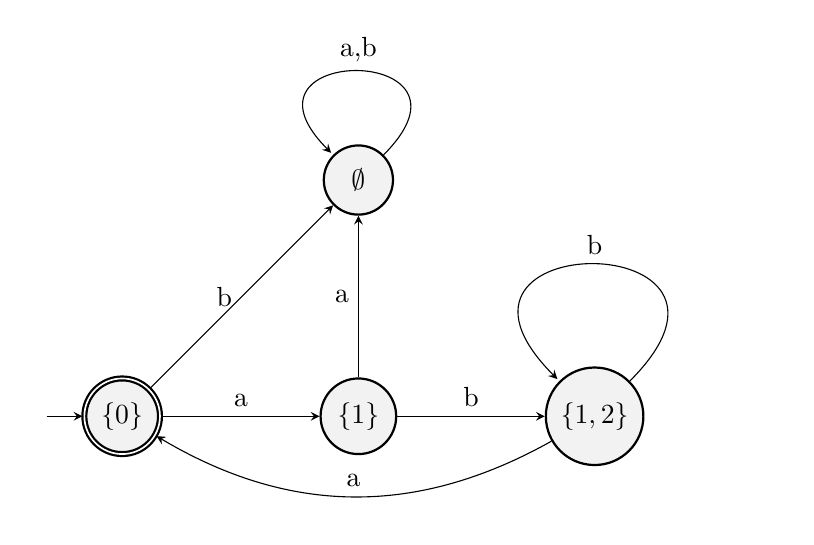
\begin{tikzpicture}
      \node[state,initial,accepting]  (q0) {$\{0\}$};
      \node[state,right of=q0]        (q1) {$\{1\}$};
      \node[state,right of=q1]        (q2) {$\{1,2\}$};
      \node[state,above of=q1]        (q3) {$\emptyset$};

      \draw (q0) edge[above]      node{a} (q1)
            (q0) edge[left]      node{b} (q3)
            (q1) edge[left]      node{a} (q3)
            (q1) edge[above]      node{b} (q2)
            (q2) edge[bend left,above]      node{a} (q0)
            (q2) edge[loop,above] node{b} (q2)
            (q3) edge[loop,above] node{a,b} (q3);
    \end{tikzpicture}
    \caption{}
    \label{fig:fig15}
\end{figure}

\subsection{Build a DFA out of an NFA by Chasing Down $\epsilon$ Transitions}

For simplicity, there are no $\epsilon$ transitions in the example in
\ref{subsec:5.1}. It takes a little more effort to deal with them. And let us
do it now. The figure below shows a slice of some NFA:

\begin{figure}[ht]
    \centering
    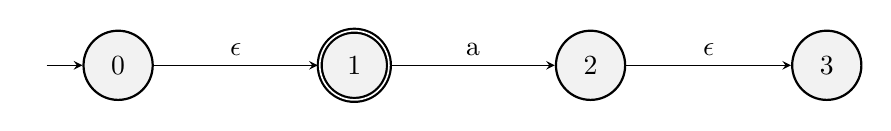
\begin{tikzpicture}
      \node[state,initial]  (q0) {0};
      \node[state,accepting,right of=q0]        (q1) {1};
      \node[state,right of=q1]        (q2) {2};
      \node[state,right of=q2]        (q3) {3};

      \draw (q0) edge[above]     node{$\epsilon$} (q1)
            (q1) edge[above]     node{a} (q2)
            (q2) edge[above]     node{$\epsilon$} (q3);
    \end{tikzpicture}
    \caption{}
    \label{fig:fig16}
\end{figure}

It takes three steps to eliminate the $\epsilon$ transitions. First, we add a
new transition to \emph{bypass} the $\epsilon$ transitions. The result is shown
is figure \ref{fig:fig16}.

\begin{figure}[ht]
    \centering
    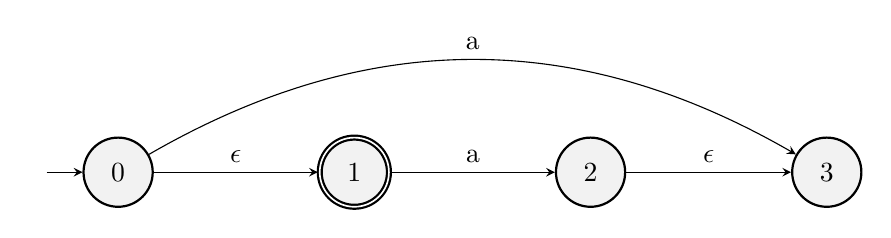
\begin{tikzpicture}
      \node[state,initial]  (q0) {0};
      \node[state,accepting,right of=q0]        (q1) {1};
      \node[state,right of=q1]        (q2) {2};
      \node[state,right of=q2]        (q3) {3};

      \draw (q0) edge[above]     node{$\epsilon$} (q1)
            (q1) edge[above]     node{a} (q2)
            (q2) edge[above]     node{$\epsilon$} (q3)
            (q0) edge[bend left,above]     node{a} (q3);
    \end{tikzpicture}
    \caption{}
    \label{fig:fig17}
\end{figure}

Then, if the $\epsilon$ transition points to an accept state, we need to turn
the start state of the $\epsilon$ transition to an accept state. The result is
shown in figure \ref{fig:fig17}.

\begin{figure}[ht]
    \centering
    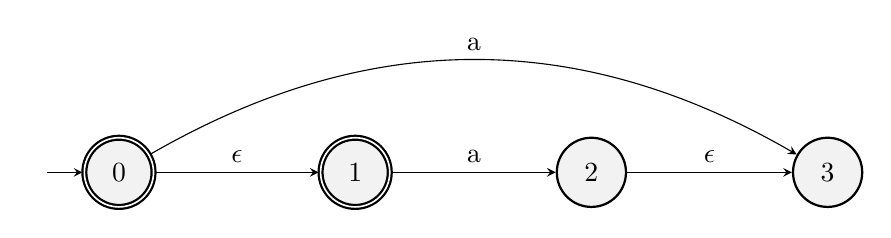
\begin{tikzpicture}
      \node[state,initial,accepting]  (q0) {0};
      \node[state,accepting,right of=q0]        (q1) {1};
      \node[state,right of=q1]        (q2) {2};
      \node[state,right of=q2]        (q3) {3};

      \draw (q0) edge[above]     node{$\epsilon$} (q1)
            (q1) edge[above]     node{a} (q2)
            (q2) edge[above]     node{$\epsilon$} (q3)
            (q0) edge[bend left,above]     node{a} (q3);
    \end{tikzpicture}
    \caption{}
    \label{fig:fig18}
\end{figure}

Finally, we can remove $\epsilon$ transtions safely. The result is shown in
figure \ref{fig:fig19}.

\begin{figure}[ht]
    \centering
    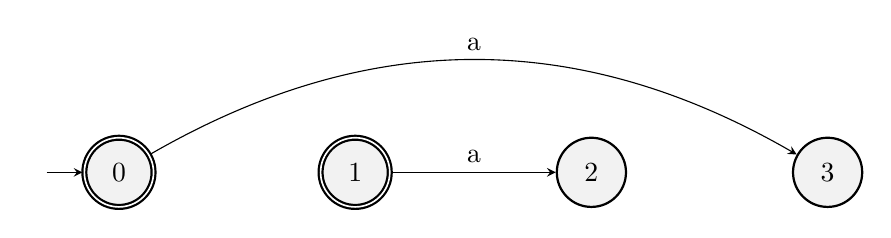
\begin{tikzpicture}
      \node[state,initial,accepting]  (q0) {0};
      \node[state,accepting,right of=q0]        (q1) {1};
      \node[state,right of=q1]        (q2) {2};
      \node[state,right of=q2]        (q3) {3};

      \draw (q1) edge[above]     node{a} (q2)
            (q0) edge[bend left,above]     node{a} (q3);
    \end{tikzpicture}
    \caption{}
    \label{fig:fig19}
\end{figure}

\subsection{Regular Language and Regular Expression}

We have seen so much about machines. Now we turn to languages and see what
languages associated with DFAs/NFAs are like.

We define a class of languages, called \emph{regular language}:
\begin{definition}
Fix the alphabet $\Sigma$. A language, $L$, is a \emph{regular language},
if either of the following is true:
\begin{enumerate}
\item $L = \emptyset$
\item $L = \{\epsilon\}$
\item $L = \{a\}$ where $a \in \Sigma$
\item $L = L_1 \cup L_2$ where $L_1$ and $L_2$ are regular languages
\item $L = L_1 \cdot L_2$ where $L_1$ and $L_2$ are regular languages
\item $L = L_1^\ast$ where $L_1$ is a regular language
\end{enumerate}
\end{definition}

It is easy to see, from the definition, that regular languages are closed
under \emph{union}, \emph{concatenation} and \emph{Kleene star}. And the
that we define it remind us of the ways to build new DFAs out of existing
ones as discussed in previous sections. There is, indeed, a connection
between regular languages and DFAs/NFAs. We will show this in next section.

It is convenient to develop a notation for regular languages, which we
call \emph{regular expressions}. We define them formally in definition
\ref{def:def19}. The regular language which is denoted by a regular
language $s$ is denoted by $L(s)$.

After the formal definition of regular languages, we specify what regular
language a regular expression \emph{matches}. Assume regular expression
$s_1$ matches $L_1$ and $s_2$ matches $L_2$, then:
\begin{enumerate}
\item $L(\epsilon) = \emptyset$
\item $L("\$\{a\}")$ = $\{a\}$
\item $L("\epsilon")$ = $\{\epsilon\}$
\item $L("(\$\{s_1\} \cup \$\{s_2\})") = L_1 \cup L_2$
\item $L("(\$\{s_1\} \cdot \$\{s_2\})") = L_1 \cdot L_2$
\item $L("(\$\{s_1\}^\ast)") = L_1 ^ \ast$
\end{enumerate}

\begin{definition} \label{def:def19}
Fix the alphabet $\Sigma$. A string $s$ over the alphabet
$\Sigma \cup \{\epsilon,(,),\cup,\cdot,\ast\}$ is a \emph{regular
expression}, if either of the following is true:
\begin{enumerate}
\item $s = \epsilon$
\item $s = "\$\{a\}"$ for some symbol $a$ in $\Sigma$
\item $s = "\epsilon"$
\item $s = "(\$\{s_1\} \cup \$\{s_2\})"$ where $s_1$ and $s_2$ are regular
expressions
\item $s = "(\$\{s_1\} \cdot \$\{s_2\})"$ where $s_1$ and $s_2$ are regular
expressions
\item $s = "(\$\{s_1\}^\ast)"$ where $s_1$ is a regular expressions
\end{enumerate}
\end{definition}

\section{DFA/NFA - Regular Language Equivalence and a Technique to Minimize a DFA}

We showed the equivalence between DFAs and NFAs. And we defined a class of
languages which we call the regular languages. In this section, we are going
to show the connection between DFAs/NFAs and regular languages. That is, the
class of languages that DFAs/NFAs accepts is exactly regular languages. There
is an equivalence between DFAs/NFAs and regular languages. We show it by
working in two directions. First, we show that for every regular expression,
we can build a DFA/NFA accepting exactly the regular language represented by
it. Then, we show that for every DFA/NFA, we can derive a regular expression
representing the language that it accepts.

\subsection{Build a DFA/NFA from a Regular Expression}

The easiest way to build a DFA/NFA from a regular expression is following
the definition of regular expressions. The base cases are shown in figure
\ref{fig:fig20} through figure \ref{fig:fig22}.

\begin{figure}[ht]
    \centering
    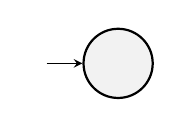
\begin{tikzpicture}
      \node[state,initial] (q0) {};
    \end{tikzpicture}
    \caption{$\emptyset$}
    \label{fig:fig20}
\end{figure}

\begin{figure}[ht]
    \centering
    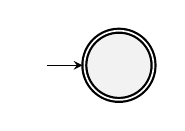
\begin{tikzpicture}
      \node[state,initial,accepting] (q0) {};
    \end{tikzpicture}
    \caption{$"\epsilon"$}
    \label{fig:fig21}
\end{figure}

\begin{figure}[ht]
    \centering
    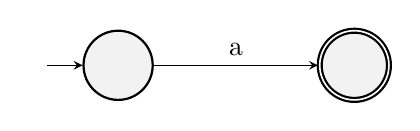
\begin{tikzpicture}
      \node[state,initial] (q0) {};
      \node[state,accepting, right of=q0] (q1) {};

      \draw (q0) edge[above] node{a} (q1);
    \end{tikzpicture}
    \caption{$"a"$}
    \label{fig:fig22}
\end{figure}

For each inductive case in the definition of regular expressions, there is
a corresponding construction of DFAs/NFAs which we discussed in detail in
section \ref{sec:3} and section \ref{sec:4}. To be specific, in the case of
$s = s_1 \cup s_2$, we use the \emph{product construction} to combine two
DFAs together. In the case of $s = s_1 \cdot s_2$, first we wire up $M_1$
and $M_2$ in the way that there are $\epsilon$ transitions connecting the
accept states of $M_1$ and the initial state of $M_2$, then we turn the
accept states of $M_1$ to nonaccept states. In the case of $s^\ast$, first
we add a new state and make it the initial state and a accept state, add
an $\epsilon$ transition from the new initial state to the original initial
state, and add $\epsilon$ transitions from the original accept states to
the original initial state.

\subsection{Derive a Regular Expression from an NFA}

To derive a regular expression from an NFA, we eliminates states from it.

First, we add a new initial state and a $\epsilon$ transition from it to
the original initial state.

Then, we add an accept state and $\epsilon$ transitions from the original
accept states to it. And we turn the original accept states to nonaccept
states.

After that, we pick a state from the original NFA and look at all paths
through it. A path should look like that shown below:

\begin{figure}[ht]
    \centering
    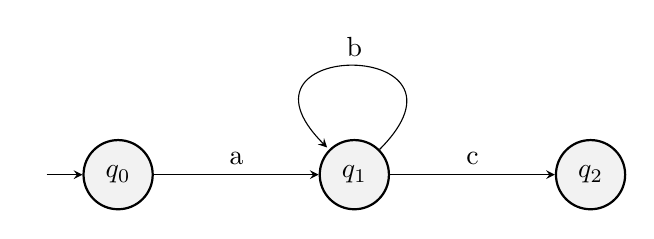
\begin{tikzpicture}
      \node[state,initial] (q0) {$q_0$};
      \node[state,right of=q0] (q1) {$q_1$};
      \node[state,right of=q1] (q2) {$q_2$};

      \draw (q0) edge[above] node{a} (q1)
            (q1) edge[loop,above] node{b} (q2)
            (q1) edge[above] node{c} (q2);
    \end{tikzpicture}
    \caption{a typical path through $q_1$}
    \label{fig:fig23}
\end{figure}

For this path, to eliminate $q_1$, we add a new transition from $q_0$ to
$q_2$, labelled by $a \cdot b^\ast c$, and remove the original transition
from $q_0$ to $q_1$ and that from $q_1$ to $q_2$. The resultant figure is
shown below:

\begin{figure}[ht]
    \centering
    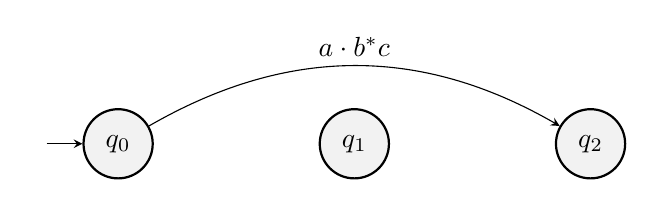
\begin{tikzpicture}
      \node[state,initial] (q0) {$q_0$};
      \node[state, right of=q0] (q1) {$q_1$};
      \node[state, right of=q1] (q2) {$q_2$};

      \draw (q0) edge[bend left,above] node{$a \cdot b^\ast c$} (q2);
    \end{tikzpicture}
    \caption{figure \ref{fig:fig23} after setting up the new transition}
    \label{fig:fig24}
\end{figure}

It should be noted that this is just one of the paths through $q_1$.
Generally, there could be many paths through $q_1$. We need to set up a
transition like this for each path. After removing original transitions
for every path, we can safely eliminate $q_1$. This process might end up
with a situation where there are two or more outgoing transitions from a
state, to one another state. An example is shown in figure \ref{fig:fig25}.

\begin{figure}[ht]
    \centering
    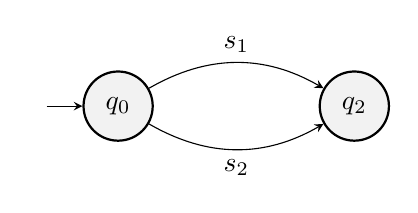
\begin{tikzpicture}
      \node[state,initial] (q0) {$q_0$};
      \node[state, right of=q0] (q2) {$q_2$};

      \draw (q0) edge[bend left,above] node{$s_1$} (q2)
            (q0) edge[bend right,below] node{$s_2$} (q2);
    \end{tikzpicture}
    \caption{a situation where there are two transitions from $q_0$ to $q_2$}
    \label{fig:fig25}
\end{figure}

In this case, we combine those outgoing transitions to a new transition
labeled by $"\$\{s_1\}\cup\$\{s_2\}"$.

\begin{figure}[ht]
    \centering
    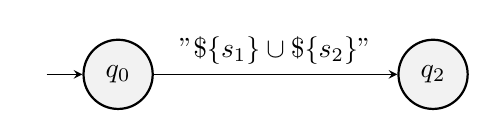
\begin{tikzpicture}
      \node[state,initial] (q0) {$q_0$};
      \node[state, right of=q0,xshift=1cm] (q2) {$q_2$};

      \draw (q0) edge[above] node{$"\$\{s_1\}\cup\$\{s_2\}"$} (q2);
    \end{tikzpicture}
    \caption{figure \ref{fig:fig25} after combining transitions}
    \label{fig:fig26}
\end{figure}

The new machine produced by the method shown above is no longer a DFA
or NFA, since the transitions are now labeled by regular expressions
instead of symbols drawn from the alphabet. We call it a \emph{generalized
nondeterministic finite automaton}. As we can imagine, after all original
states are eliminated, there would be two states and a transition between
them left. The label of the transition is the regular expression
representing the language which the original DFA/NFA accepts.

\subsection{A Technique to Minimize a DFA}

To minimize a DFA, we find \emph{equivalent states} and combine them.
What does it mean for states to be equivalent? For a DFA $M$, imagine
two states $q_0$ and $q_1$ of it. If $\delta(q_0, x) = \delta(q_1, x)$
holds for any string $x$, it makes no difference whether $M$ is in $q_0$
or $q_1$. So we can eliminate one of them and migrate all its ingoing
transitions to the other one.

This is better explained in an example. Consider the DFA shown below:

\begin{figure}[ht]
    \centering
    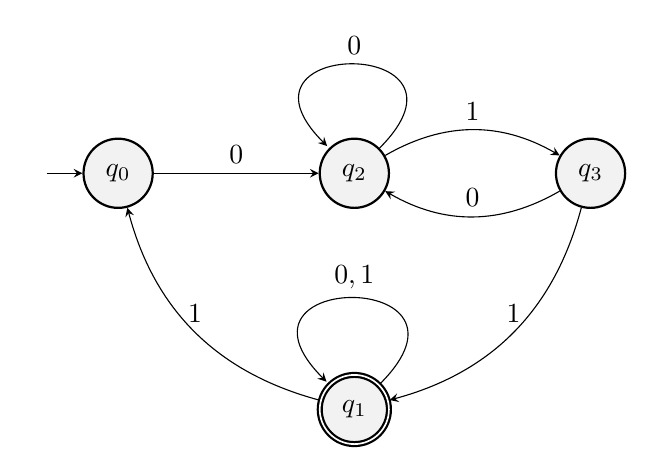
\begin{tikzpicture}
      \node[state,initial] (q0) {$q_0$};
      \node[state,right of=q0] (q2) {$q_2$};
      \node[state,accepting,below of=q2] (q1) {$q_1$};
      \node[state,right of=q2] (q3) {$q_3$};

      \draw (q0) edge[above] node{$0$} (q2)
            (q2) edge[loop,above] node{$0$} (q2)
            (q2) edge[bend left,above] node{$1$} (q3)
            (q3) edge[bend left,above] node{$0$} (q2)
            (q3) edge[bend left,above] node{$1$} (q1)
            (q1) edge[loop,above] node{$0,1$} (q1)
            (q1) edge[bend left,above] node{$1$} (q0);
    \end{tikzpicture}
    \caption{figure \ref{fig:fig25} after combining transitions}
    \label{fig:fig27}
\end{figure}

Which states should be considered equivalent? $q_1$ is not equivalent
to any other states since it is an accept state. $q_0$ is not
equivalent to $q_2$ because input $1$ takes $q_0$ to $q_2$ but takes
$q_2$ to $q_3$. $q_2$ is not equivalent to $q_3$ because input $1$
takes $q_2$ to $q_3$ but takes $q_3$ to $q_1$. $q_0$ is equivalent to
$q_3$ because both inputs $0$ and $1$ take them to the same states.
We decide to eliminate $q_3$. To do so, first we migrate all its
ingoing transitions to $q_0$. There is one ingoing transition from $q_2$.
So we add a new transition from $q_2$ to $q_0$ labeled by $1$. And we
remove $q_3$ together with all transitions associated with it. This
yields the DFA shown below:

\begin{figure}[ht]
    \centering
    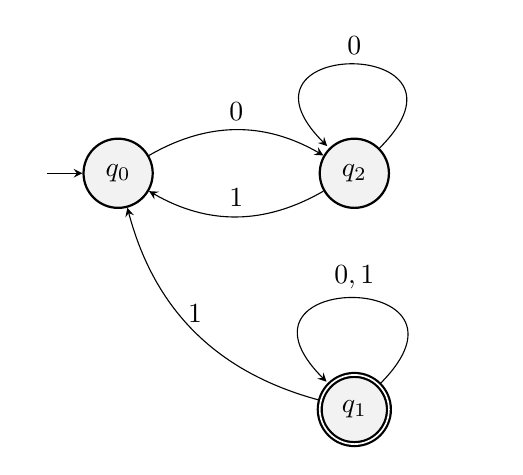
\begin{tikzpicture}
      \node[state,initial] (q0) {$q_0$};
      \node[state,right of=q0] (q2) {$q_2$};
      \node[state,accepting,below of=q2] (q1) {$q_1$};

      \draw (q0) edge[bend left,above] node{$0$} (q2)
            (q2) edge[loop,above] node{$0$} (q2)
            (q2) edge[bend left,above] node{$1$} (q0)
            (q1) edge[loop,above] node{$0,1$} (q1)
            (q1) edge[bend left,above] node{$1$} (q0);
    \end{tikzpicture}
    \caption{minimized version of figure \ref{fig:fig27}}
    \label{fig:fig28}
\end{figure}

\end{document}
